\documentclass{standalone}
\usepackage{tikz}
\usepackage{ctex,siunitx}
\setCJKmainfont{Noto Serif CJK SC}
\usepackage{tkz-euclide}
\usepackage{amsmath}
\usetikzlibrary{patterns, calc,3d}
\usetikzlibrary {decorations.pathmorphing,decorations.pathreplacing,decorations.shapes}
\begin{document}
\small
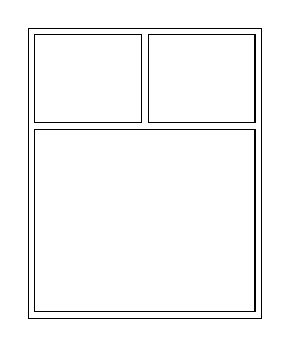
\begin{tikzpicture}[>=latex,scale=0.8]
  \draw[double,double distance=2pt](0,0)rectangle(3.6,4.5)(0,3)--(3.6,3)(1.8,3)--(1.8,4.5);
\end{tikzpicture}
\end{document}